\chapter{Appendices}
\section{Exploratory Survey}

\section*{Questionnaire}

\begin{enumerate}

    % Question 1
    \item \textbf{When was the last time you played Wordle?} \\
    Please select one option:
    \begin{itemize}
        \item I play every day
        \item I have played at least once in the last week
        \item I have played at least once in the last month
        \item I have played at least once in the last two months
        \item I have played at least once in the last six months
        \item I have played Wordle at least once since release
        \item I have never played Wordle
    \end{itemize}

    % Question 2
    \item \textbf{Which option best describes you?} \\
    Please select one option:
    \begin{itemize}
        \item I play Wordle daily.
        \item I used to play Wordle daily but now I play less frequently.
        \item I used to play Wordle daily but no longer play.
        \item I play Wordle occasionally.
        \item I used to play Wordle occasionally but have stopped.
        \item I have never played Wordle.
    \end{itemize}

    % Question 3
    \item \textbf{If you no longer play Wordle, could you please share the reasons why?} \\
    \textit{Enter your answer:} \underline{\hspace{10cm}}

    % Question 4
    \item \textbf{What could make you start playing Wordle again if you've stopped?} \\
    Please select one option:
    \begin{itemize}
        \item New features or updates
        \item More challenging puzzles
        \item Playing with friends/family
        \item I’m unlikely to start playing again
        \item Other: \underline{\hspace{5cm}}
    \end{itemize}

    % Question 5
    \item \textbf{How long would you typically spend on Wordle in a day?} \\
    Please select one option:
    \begin{itemize}
        \item Less than 5 minutes
        \item 5-10 minutes
        \item 10-20 minutes
        \item More than 20 minutes
        \item It varies depending on the difficulty
    \end{itemize}

    % Question 6
    \item \textbf{Would you be interested in additional Wordle content or variations?} \\
    Please select one option:
    \begin{itemize}
        \item Yes, I would like more variations
        \item No, I prefer the original game
        \item No, I’m not interested in variations
    \end{itemize}

    % Question 7
    \item \textbf{How happy are you with the current version of Wordle?} \\
    \textit{Please rate your satisfaction on a scale of 1 to 10 (1 = not happy at all, 10 = extremely happy):}
    \begin{itemize}
        \item 1
        \item 2
        \item 3
        \item 4
        \item 5
        \item 6
        \item 7
        \item 8
        \item 9
        \item 10
    \end{itemize}

\end{enumerate}

\section{Questionnaire Results}
\begin{figure}[h] % 'h' means 'here' - places the figure where it's defined
    \centering
    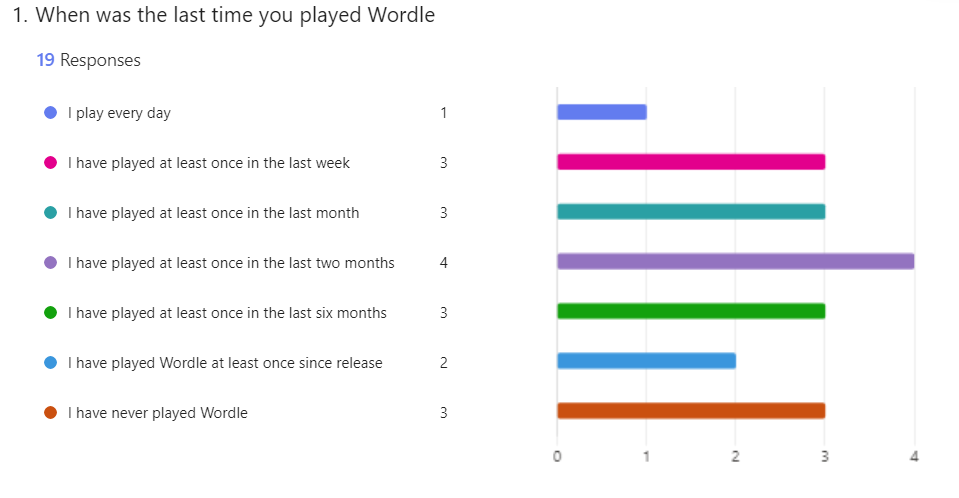
\includegraphics[width=\textwidth]{WordleResponse1.png} % Replace with your image file
    \label{fig:example}
\end{figure}
\begin{figure}[h] % 'h' means 'here' - places the figure where it's defined
    \centering
    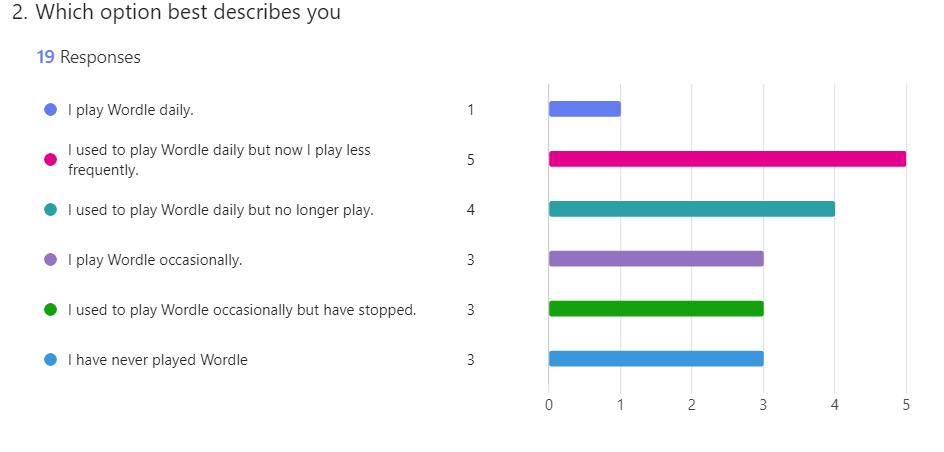
\includegraphics[width=\textwidth]{WordleResponse2.png} % Replace with your image file
    \label{fig:example}
\end{figure}
\begin{figure}[h] % 'h' means 'here' - places the figure where it's defined
    \centering
    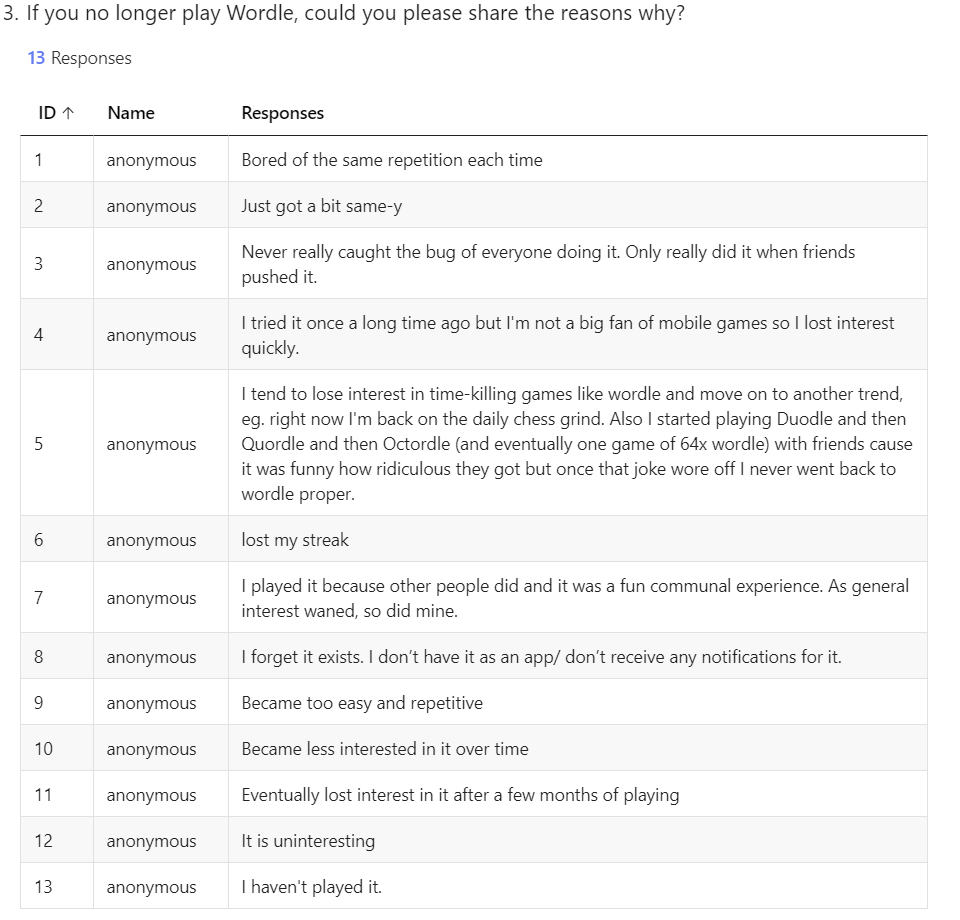
\includegraphics[width=\textwidth]{WordleResponse3.png} % Replace with your image file
    \label{fig:example}
\end{figure}
\begin{figure}[h] % 'h' means 'here' - places the figure where it's defined
    \centering
    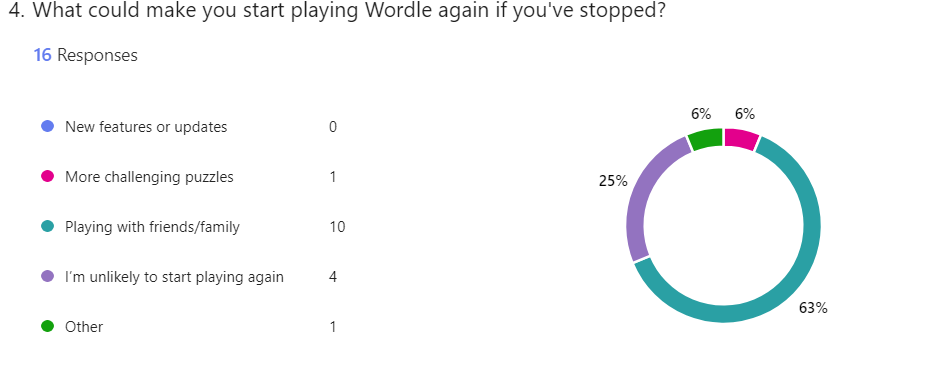
\includegraphics[width=\textwidth]{WordleResponse4.png} % Replace with your image file
    \label{fig:example}
\end{figure}
\begin{figure}[h] % 'h' means 'here' - places the figure where it's defined
    \centering
    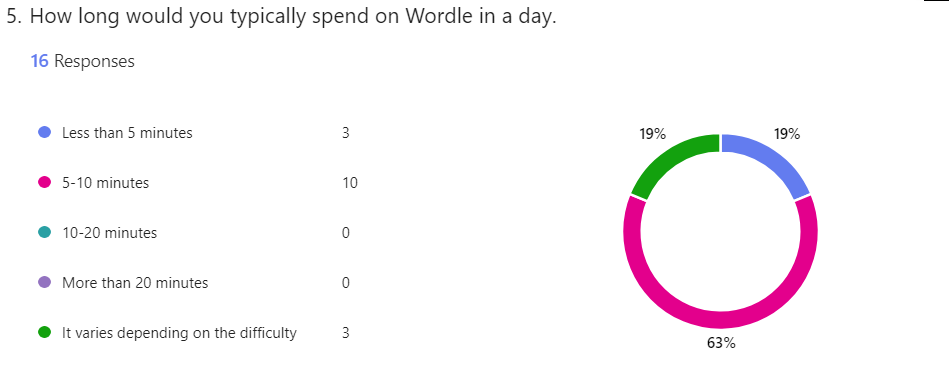
\includegraphics[width=\textwidth]{WordleResponse5.png} % Replace with your image file
    \label{fig:example}
\end{figure}
\begin{figure}[h] % 'h' means 'here' - places the figure where it's defined
    \centering
    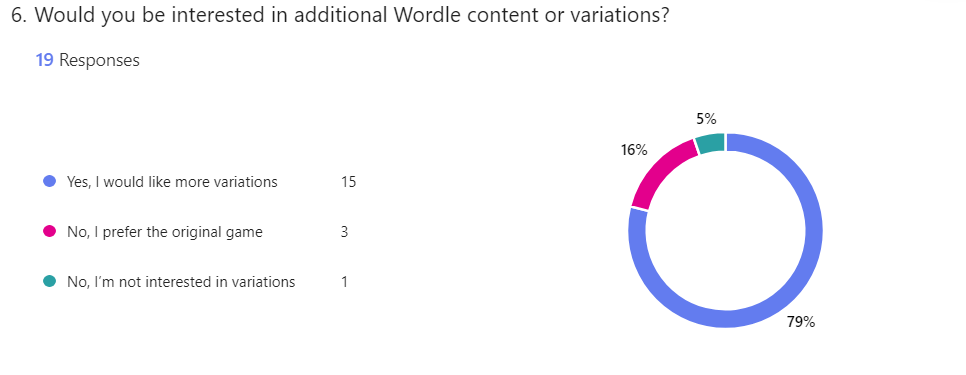
\includegraphics[width=\textwidth]{WordleResponse6.png} % Replace with your image file
    \label{fig:example}
\end{figure}
\begin{figure}[h] % 'h' means 'here' - places the figure where it's defined
    \centering
    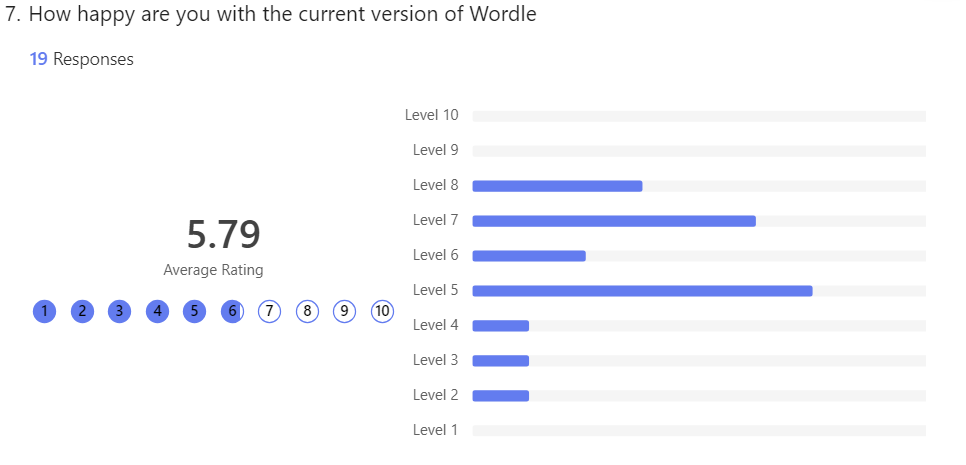
\includegraphics[width=\textwidth]{WordleResponse7.png} % Replace with your image file
    \label{fig:example}
\end{figure}
\clearpage
\section{The Gauntlet Exit Form}

\begin{enumerate}
    \item \textbf{What is your name?} \\
    \textit{(Enter your answer below.)}
    \vspace{2cm}
    \hrulefill
    
    \item \textbf{How much did you enjoy The Gauntlet (Wordle with more features)?} \\
    (On a scale of 1 to 5, with 1 being not enjoyable and 5 being very enjoyable.)
    \begin{enumerate}[label=(\arabic*)]
        \item 1
        \item 2
        \item 3
        \item 4
        \item 5
    \end{enumerate}

    \item \textbf{How much did you enjoy Wordle with increased word length?}
    \begin{enumerate}[label=(\arabic*)]
        \item 1
        \item 2
        \item 3
        \item 4
        \item 5
    \end{enumerate}

    \item \textbf{How frustrating did you find Wordle with increased word length?}
    \begin{enumerate}[label=(\arabic*)]
        \item 1
        \item 2
        \item 3
        \item 4
        \item 5
    \end{enumerate}

    \item \textbf{How much did you enjoy the Leaderboards feature?}
    \begin{enumerate}[label=(\arabic*)]
        \item 1
        \item 2
        \item 3
        \item 4
        \item 5
    \end{enumerate}

    \item \textbf{How much did you enjoy the achievements feature?}
    \begin{enumerate}[label=(\arabic*)]
        \item 1
        \item 2
        \item 3
        \item 4
        \item 5
    \end{enumerate}

    \item \textbf{How much did you enjoy the shared game feature?}
    \begin{enumerate}[label=(\arabic*)]
        \item 1
        \item 2
        \item 3
        \item 4
        \item 5
    \end{enumerate}

    \item \textbf{Do you believe the Leaderboard encouraged you to play more?}
    \begin{enumerate}[label=(\arabic*)]
        \item Yes
        \item No
    \end{enumerate}

    \item \textbf{Please explain why.}
    \vspace{2cm}
    \hrulefill

    \item \textbf{Do you believe the Achievement system encouraged you to play more?}
    \begin{enumerate}[label=(\arabic*)]
        \item Yes
        \item No
    \end{enumerate}

    \item \textbf{Please explain why.}
    \vspace{2cm}
    \hrulefill

    \item \textbf{Did the Shared game feature encourage you to play more?}
    \begin{enumerate}[label=(\arabic*)]
        \item Yes
        \item No
    \end{enumerate}

    \item \textbf{Please explain why.}
    \vspace{2cm}
    \hrulefill

    \item \textbf{Were you aware what the Share button did at the end of each game?}
    \begin{enumerate}[label=(\arabic*)]
        \item Yes
        \item No
    \end{enumerate}

    \item \textbf{Which of the additional features encouraged you to play the most?}
    \begin{enumerate}[label=(\arabic*)]
        \item Achievements
        \item Leaderboard
        \item Sharing your game
        \item Increased word length Wordle
    \end{enumerate}

    \item \textbf{Was there any feature you wish hadn't been included?}
    \begin{enumerate}[label=(\arabic*)]
        \item Achievements
        \item Leaderboard
        \item Shared
        \item Increased word length
        \item I was fine with all the features
    \end{enumerate}

    \item \textbf{If you chose a feature you wish wasn't on the website, please explain why.}
    \vspace{2cm}
    \hrulefill

    \item \textbf{Is there any other feature you would have liked to have added?}
    \vspace{2cm}
    \hrulefill

    \item \textbf{Did you play on your phone at any point during the experiment?}
    \begin{enumerate}[label=(\arabic*)]
        \item Yes
        \item No
    \end{enumerate}

    \item \textbf{When using the stripped-down Wordle, did you miss the features that were added in The Gauntlet?}
    \begin{enumerate}[label=(\arabic*)]
        \item Yes
        \item No
    \end{enumerate}

    \item \textbf{Did you prefer stripped-down Wordle or Wordle with more features?}
    \begin{enumerate}[label=(\arabic*)]
        \item Wordle
        \item Wordle with more features
    \end{enumerate}

    \item \textbf{Do you find Wordle with 5 letters challenging?}
    \begin{enumerate}[label=(\arabic*)]
        \item Yes
        \item No
    \end{enumerate}

    \item \textbf{If no, did the increased word length feel appropriately challenging? Please explain.}
    \vspace{2cm}
    \hrulefill

    \item \textbf{Did you encounter any issues when using either websites?}
    \vspace{2cm}
    \hrulefill

\end{enumerate}

\section{The Gauntlet Exit Form Results}
\begin{figure}[h] % 'h' means 'here' - places the figure where it's defined
    \centering
    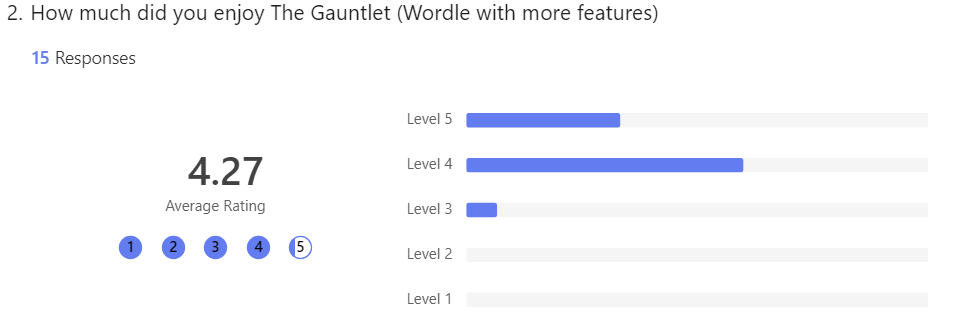
\includegraphics[width=\textwidth]{GauntletResponse1.png} % Replace with your image file
    \label{fig:example}
\end{figure}
\begin{figure}[h] % 'h' means 'here' - places the figure where it's defined
    \centering
    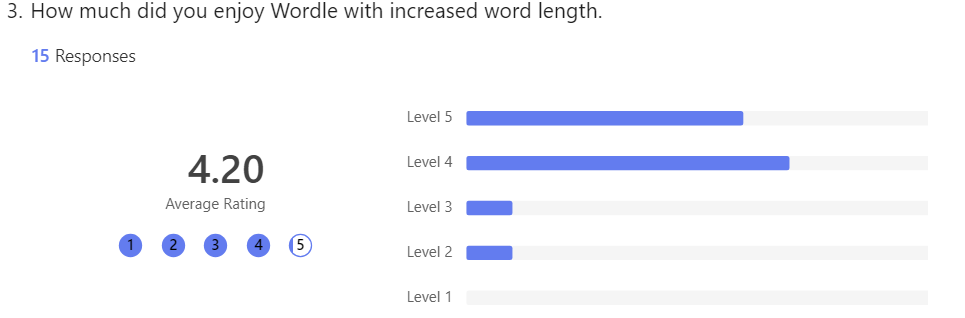
\includegraphics[width=\textwidth]{GauntletResponse2.png} % Replace with your image file
    \label{fig:example}
\end{figure}
\begin{figure}[h] % 'h' means 'here' - places the figure where it's defined
    \centering
    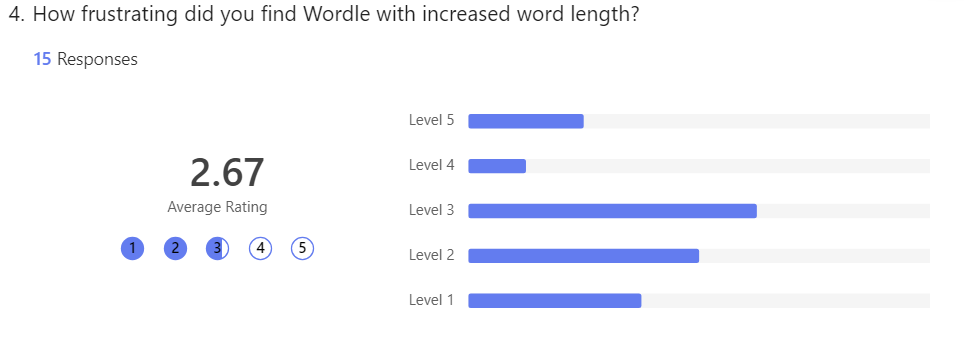
\includegraphics[width=\textwidth]{GauntletResponse3.png} % Replace with your image file
    \label{fig:example}
\end{figure}
\begin{figure}[h] % 'h' means 'here' - places the figure where it's defined
    \centering
    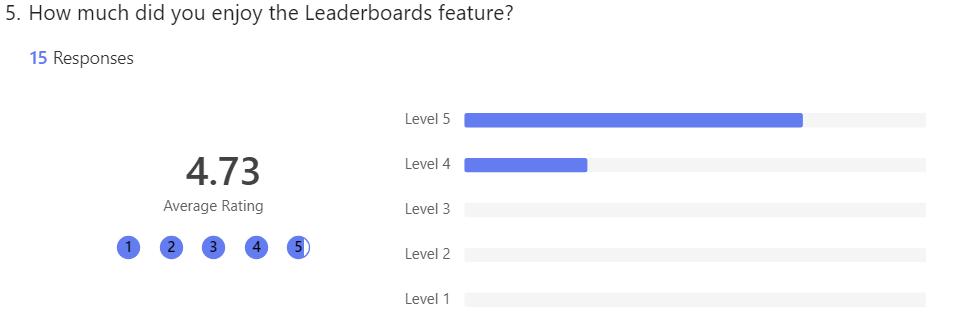
\includegraphics[width=\textwidth]{GauntletResponse4.png} % Replace with your image file
    \label{fig:example}
\end{figure}
\begin{figure}[h] % 'h' means 'here' - places the figure where it's defined
    \centering
    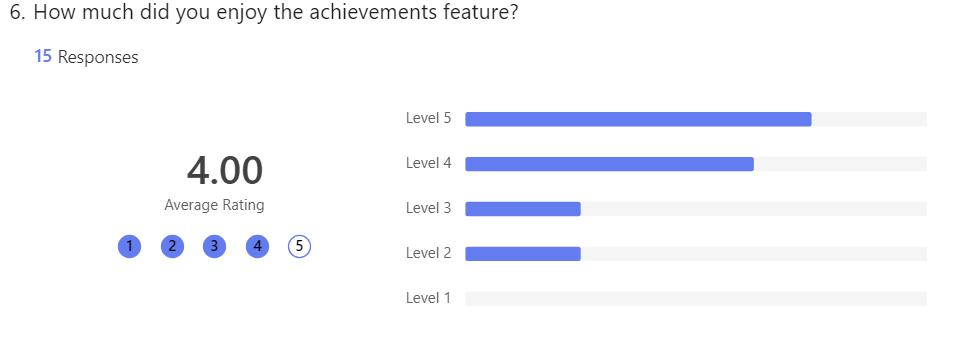
\includegraphics[width=\textwidth]{GauntletResponse5.png} % Replace with your image file
    \label{fig:example}
\end{figure}
\begin{figure}[h] % 'h' means 'here' - places the figure where it's defined
    \centering
    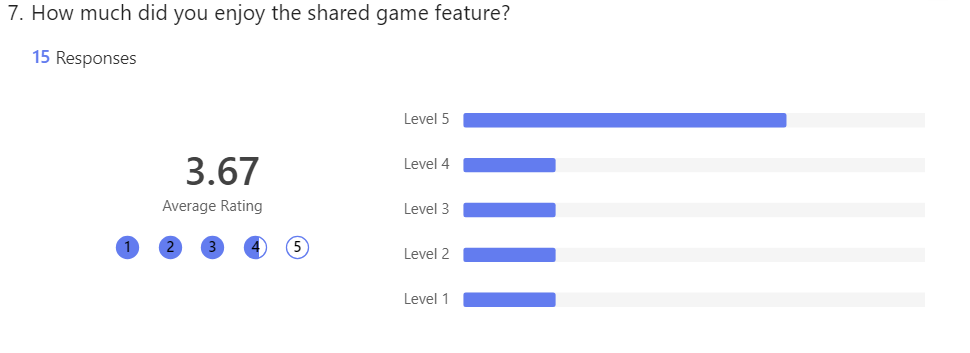
\includegraphics[width=\textwidth]{GauntletResponse6.png} % Replace with your image file
    \label{fig:example}
\end{figure}
\begin{figure}[h] % 'h' means 'here' - places the figure where it's defined
    \centering
    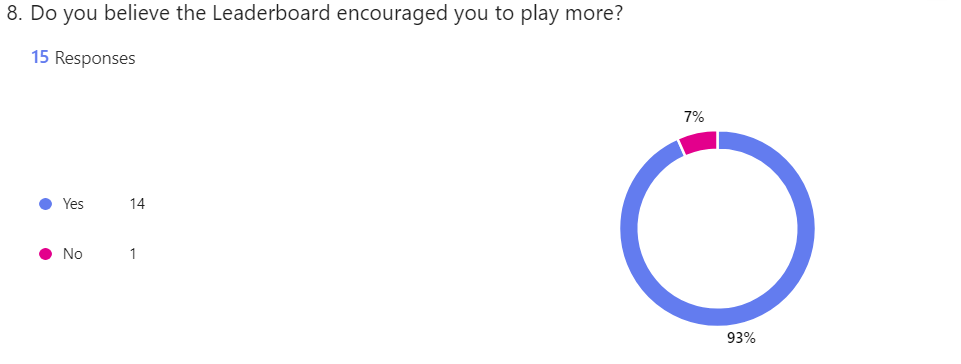
\includegraphics[width=\textwidth]{GauntletResponse7.png} % Replace with your image file
    \label{fig:example}
\end{figure}
\begin{figure}[h] % 'h' means 'here' - places the figure where it's defined
    \centering
    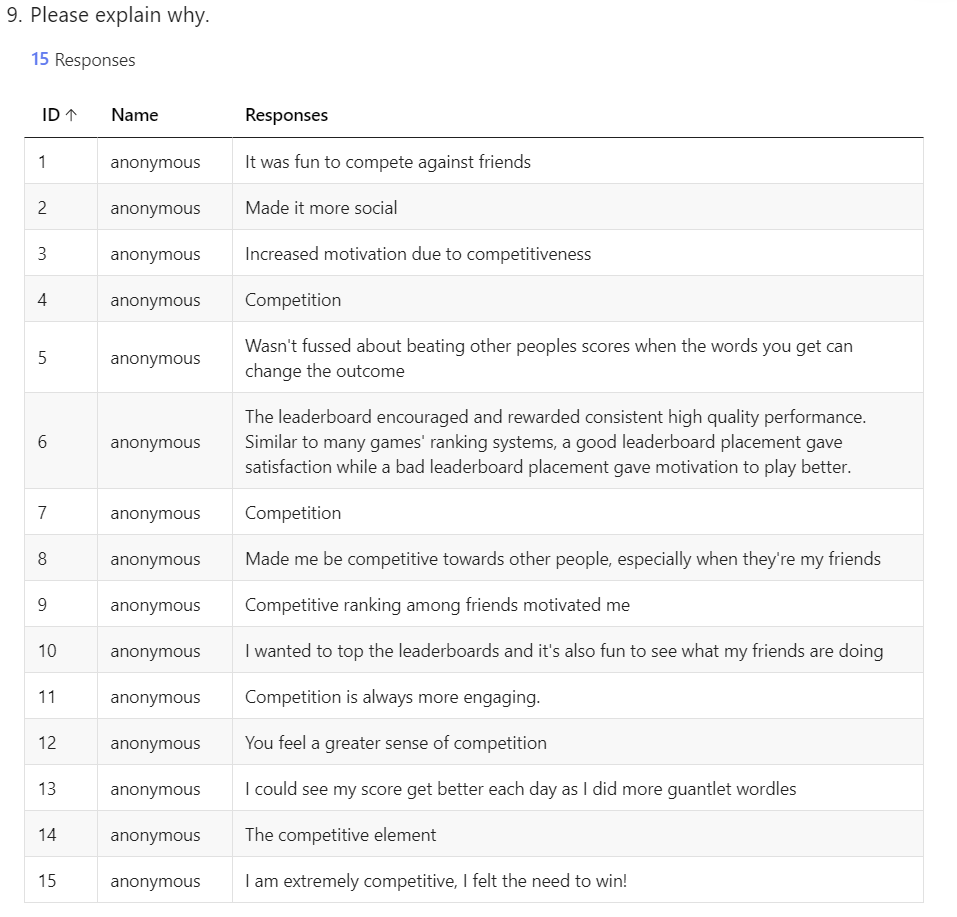
\includegraphics[width=\textwidth]{GauntletResponse8.png} % Replace with your image file
    \label{fig:example}
\end{figure}
\begin{figure}[h] % 'h' means 'here' - places the figure where it's defined
    \centering
    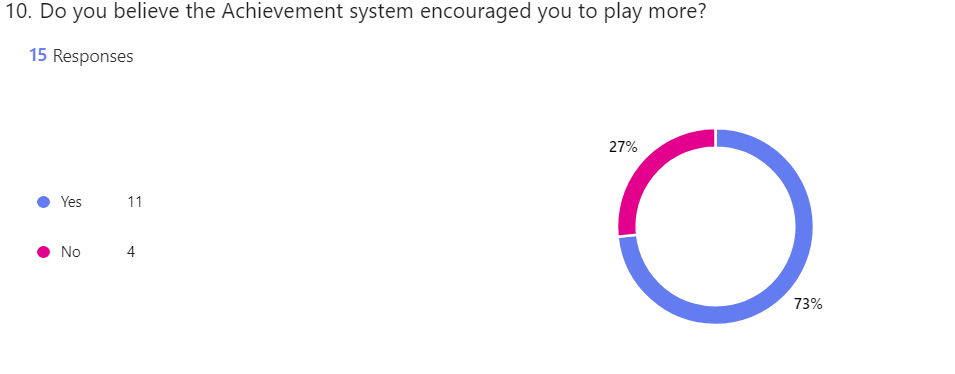
\includegraphics[width=\textwidth]{GauntletResponse9.png} % Replace with your image file
    \label{fig:example}
\end{figure}
\begin{figure}[h] % 'h' means 'here' - places the figure where it's defined
    \centering
    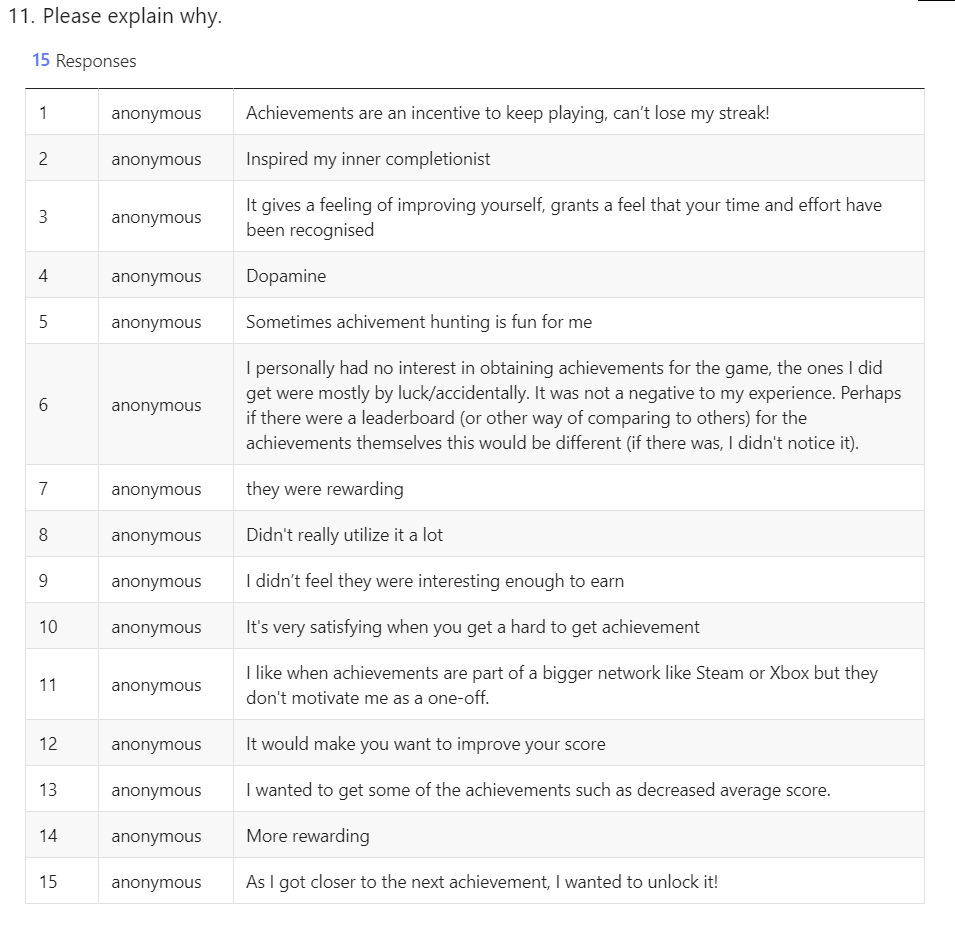
\includegraphics[width=\textwidth]{GauntletResponse10.png} % Replace with your image file
    \label{fig:example}
\end{figure}
\begin{figure}[h] % 'h' means 'here' - places the figure where it's defined
    \centering
    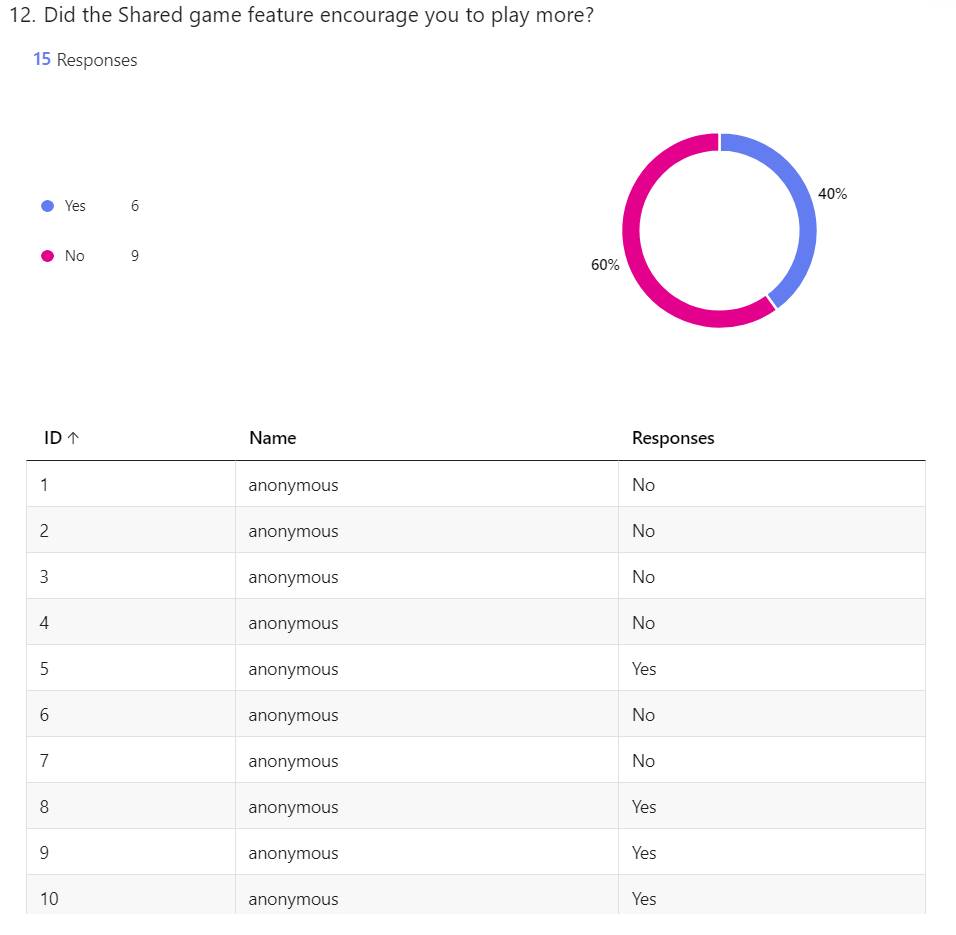
\includegraphics[width=\textwidth]{GauntletResponse11.png} % Replace with your image file
    \label{fig:example}
\end{figure}
\begin{figure}[h] % 'h' means 'here' - places the figure where it's defined
    \centering
    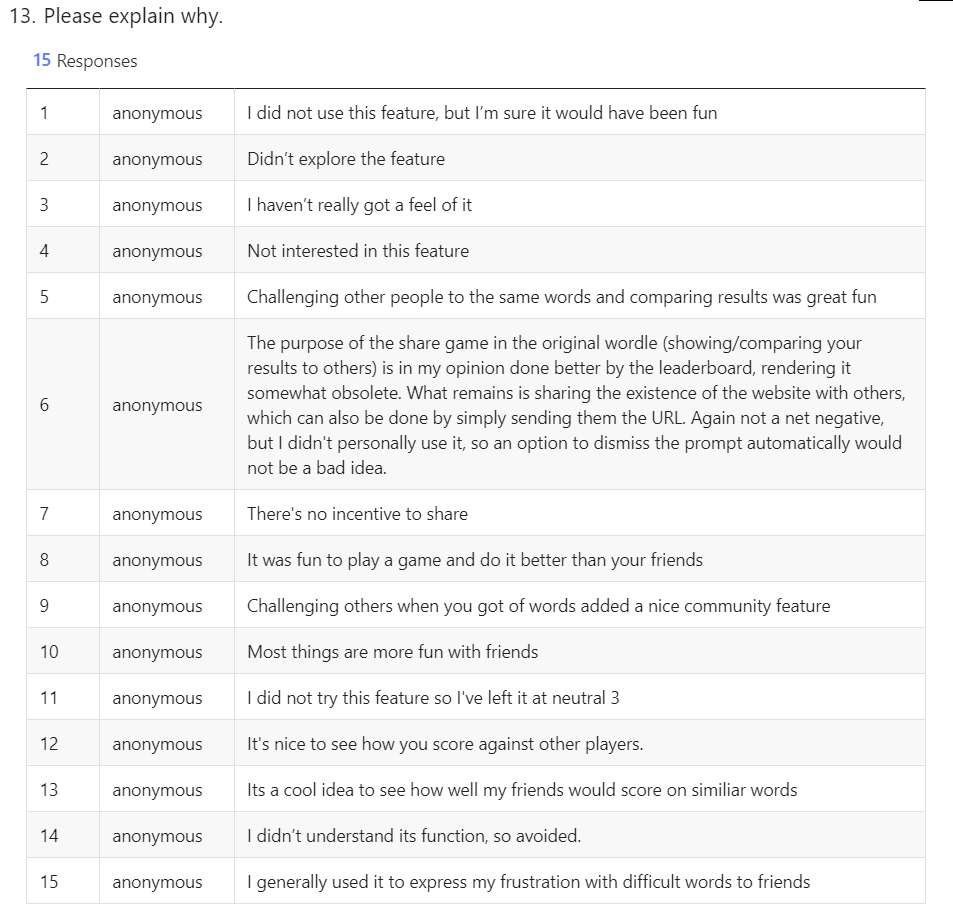
\includegraphics[width=\textwidth]{GauntletResponse12.png} % Replace with your image file
    \label{fig:example}
\end{figure}
\begin{figure}[h] % 'h' means 'here' - places the figure where it's defined
    \centering
    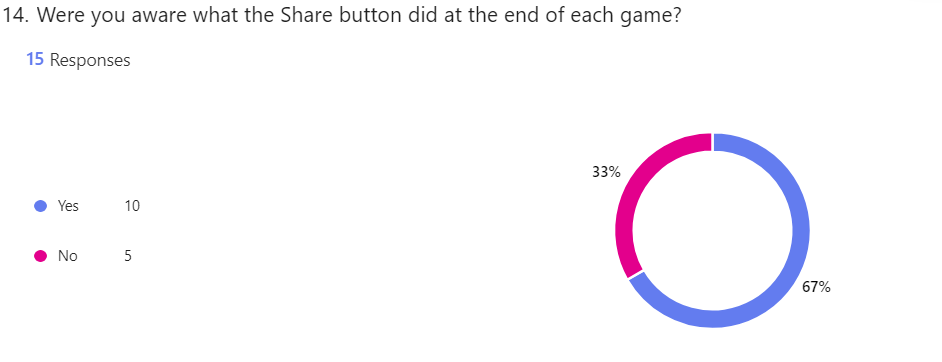
\includegraphics[width=\textwidth]{GauntletResponse13.png} % Replace with your image file
    \label{fig:example}
\end{figure}
\begin{figure}[h] % 'h' means 'here' - places the figure where it's defined
    \centering
    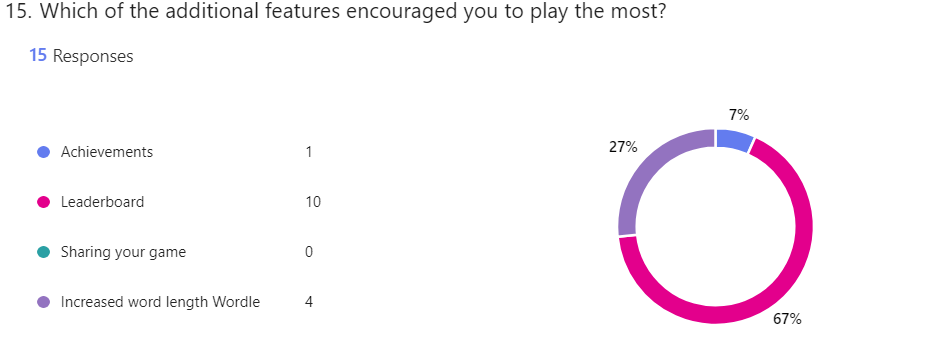
\includegraphics[width=\textwidth]{GauntletResponse14.png} % Replace with your image file
    \label{fig:example}
\end{figure}
\begin{figure}[h] % 'h' means 'here' - places the figure where it's defined
    \centering
    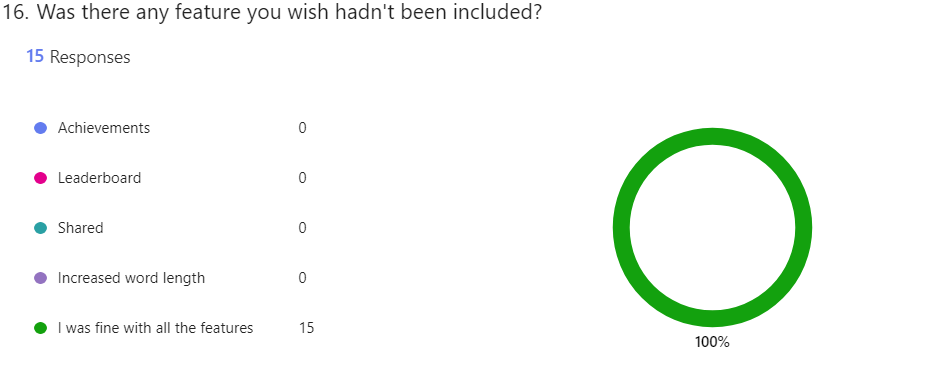
\includegraphics[width=\textwidth]{GauntletResponse15.png} % Replace with your image file
    \label{fig:example}
\end{figure}
\begin{figure}[h] % 'h' means 'here' - places the figure where it's defined
    \centering
    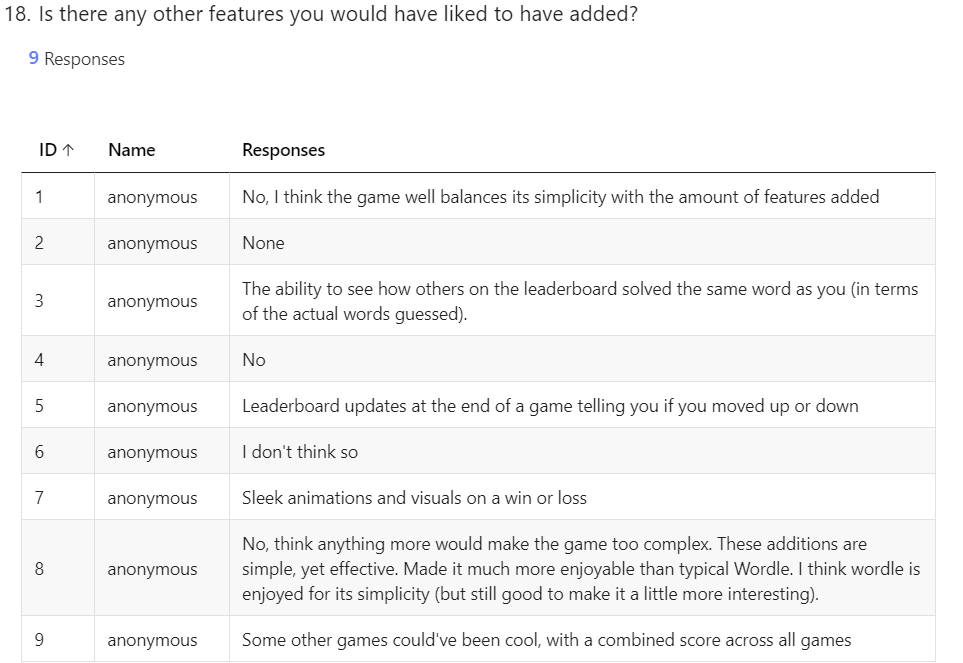
\includegraphics[width=\textwidth]{GauntletResponse16.png} % Replace with your image file
    \label{fig:example}
\end{figure}
\begin{figure}[h] % 'h' means 'here' - places the figure where it's defined
    \centering
    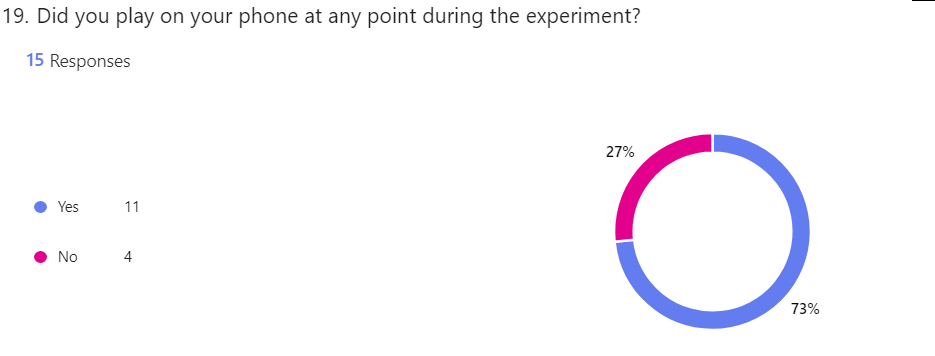
\includegraphics[width=\textwidth]{GauntletResponse17.png} % Replace with your image file
    \label{fig:example}
\end{figure}
\begin{figure}[h] % 'h' means 'here' - places the figure where it's defined
    \centering
    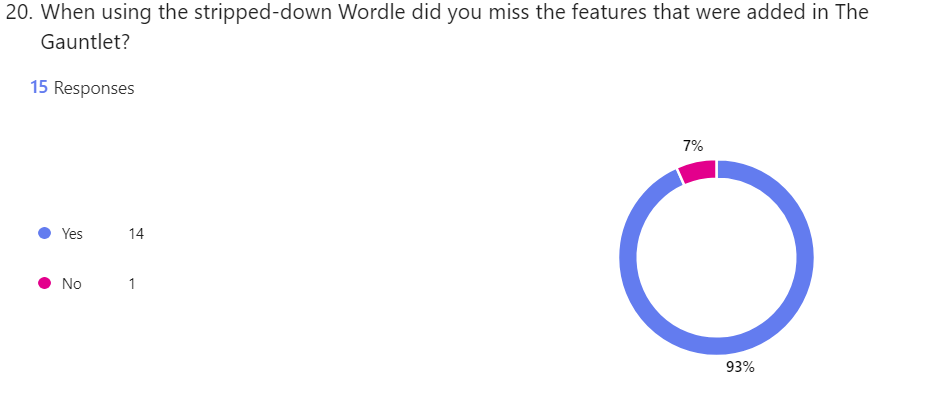
\includegraphics[width=\textwidth]{GauntletResponse18.png} % Replace with your image file
    \label{fig:example}
\end{figure}
\begin{figure}[h] % 'h' means 'here' - places the figure where it's defined
    \centering
    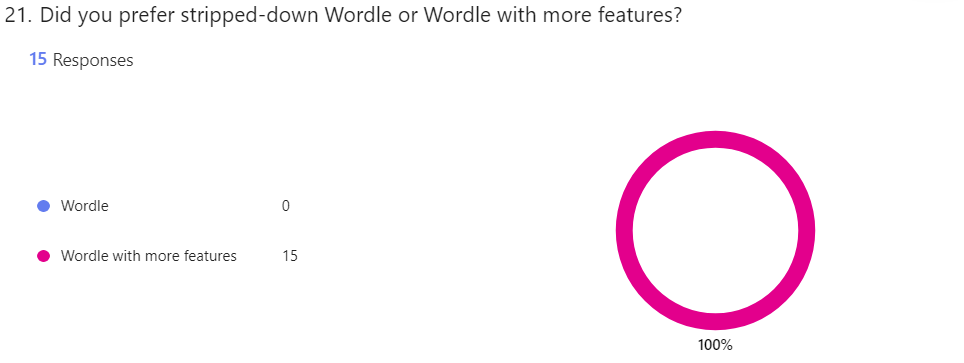
\includegraphics[width=\textwidth]{GauntletResponse19.png} % Replace with your image file
    \label{fig:example}
\end{figure}
\begin{figure}[h] % 'h' means 'here' - places the figure where it's defined
    \centering
    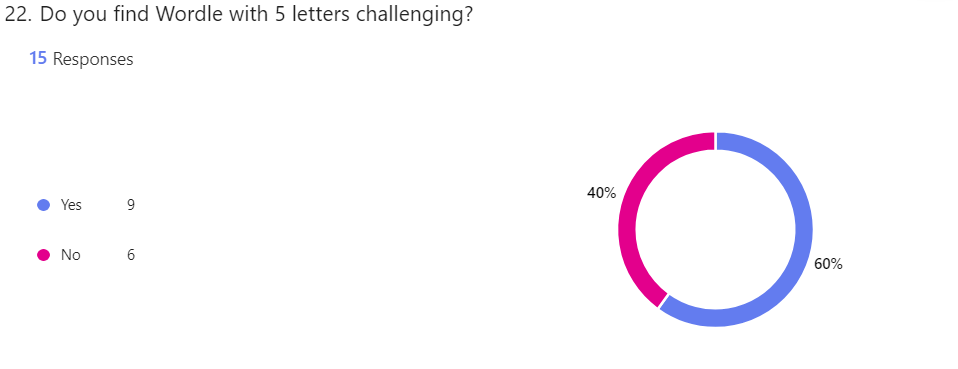
\includegraphics[width=\textwidth]{GauntletResponse20.png} % Replace with your image file
    \label{fig:example}
\end{figure}
\begin{figure}[h] % 'h' means 'here' - places the figure where it's defined
    \centering
    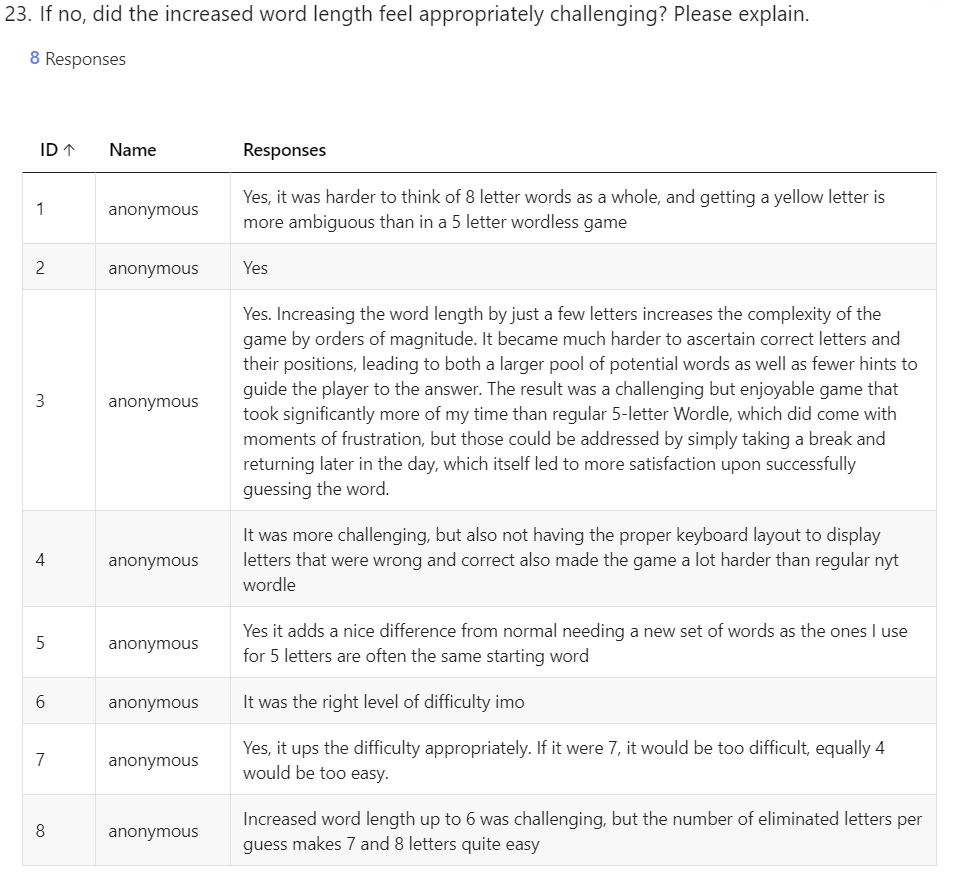
\includegraphics[width=\textwidth]{GauntletResponse21.png} % Replace with your image file
    \label{fig:example}
\end{figure}
\begin{figure}[h] % 'h' means 'here' - places the figure where it's defined
    \centering
    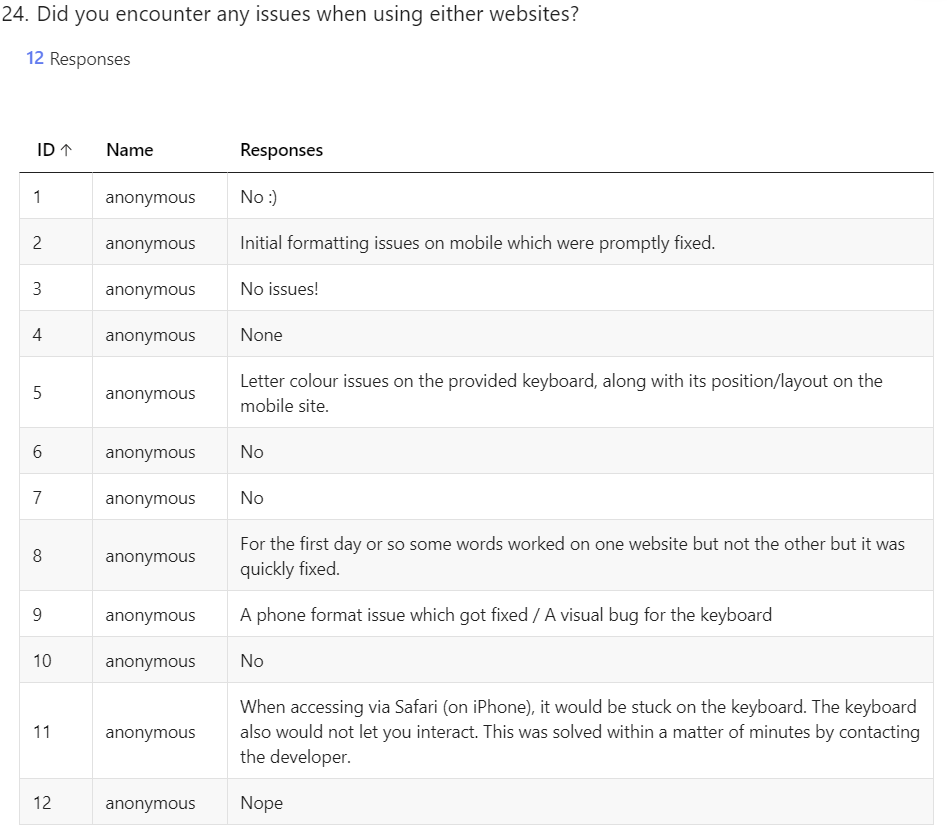
\includegraphics[width=\textwidth]{GauntletResponse22.png} % Replace with your image file
    \label{fig:example}
\end{figure}
\clearpage

\section{Google Analytics Result}
\begin{figure}[h] % 'h' means 'here' - places the figure where it's defined
    \centering
    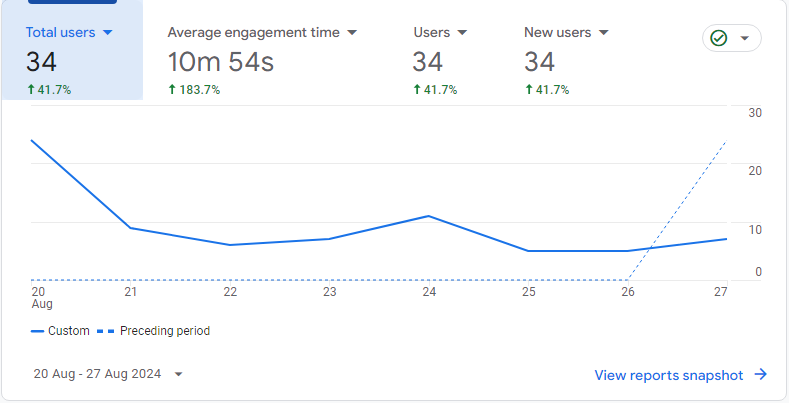
\includegraphics[width=\textwidth]{GoogleAnalytics1.png} % Replace with your image file
    \label{fig:example}
    \caption{Graph of the total users each day for The Gauntlet}
\end{figure}
\begin{figure}[h] % 'h' means 'here' - places the figure where it's defined
    \centering
    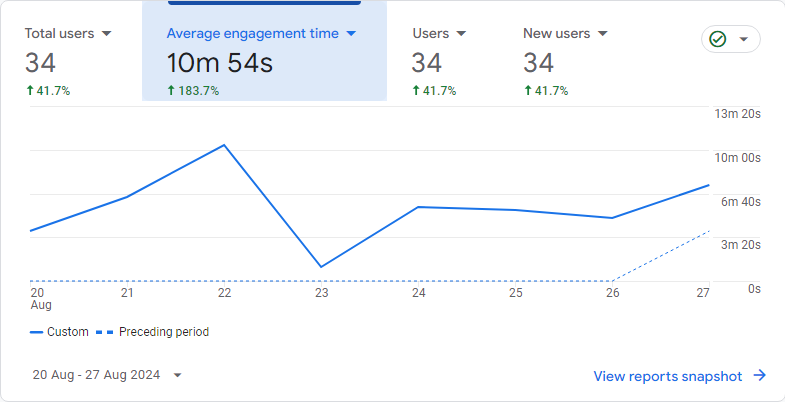
\includegraphics[width=\textwidth]{GoogleAnalytics2.png} % Replace with your image file
    \label{fig:example}
    \caption{Graph of average engagement time each day for The Gauntlet}
\end{figure}
\begin{figure}[h] % 'h' means 'here' - places the figure where it's defined
    \centering
    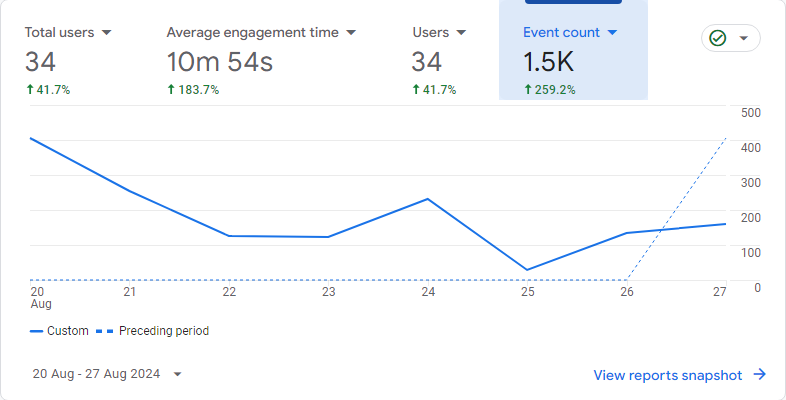
\includegraphics[width=\textwidth]{GoogleAnalytics3.png} % Replace with your image file
    \label{fig:example}
    \caption{Graph of event count each day for The Gauntlet}
\end{figure}
\begin{figure}[h] % 'h' means 'here' - places the figure where it's defined
    \centering
    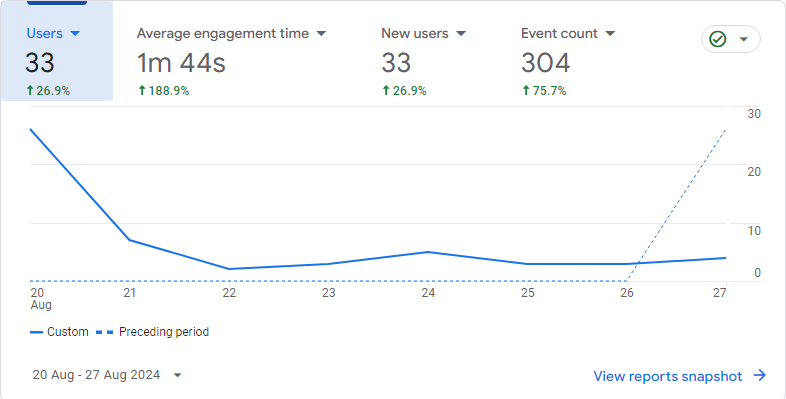
\includegraphics[width=\textwidth]{GoogleAnalytics4.png} % Replace with your image file
    \label{fig:example}
    \caption{Graph of total users each day for Wordle no-login}
\end{figure}
\begin{figure}[h] % 'h' means 'here' - places the figure where it's defined
    \centering
    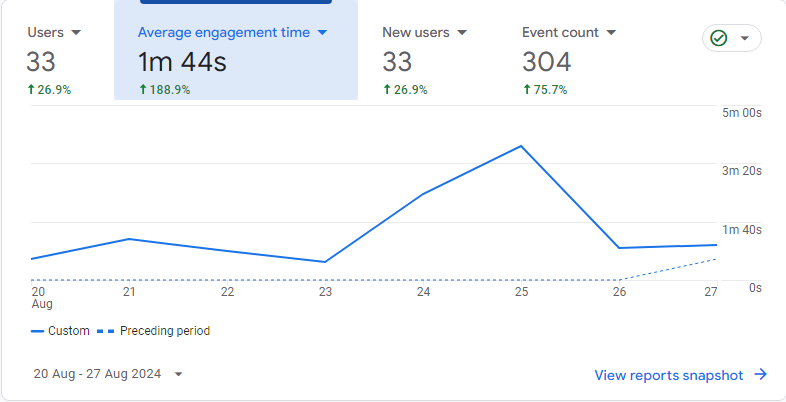
\includegraphics[width=\textwidth]{GoogleAnalytics5.png} % Replace with your image file
    \label{fig:example}
    \caption{Graph of average engagement time each day for Wordle no-login}
\end{figure}
\begin{figure}[h] % 'h' means 'here' - places the figure where it's defined
    \centering
    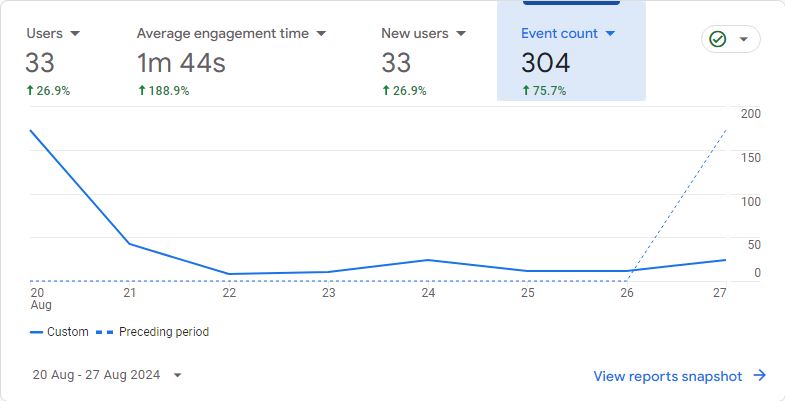
\includegraphics[width=\textwidth]{GoogleAnalytics6.png} % Replace with your image file
    \label{fig:example}
    \caption{Graph of event count each day for Wordle no-login}
\end{figure}